\documentclass[10pt,a4paper]{ctexart}
\usepackage[margin=2cm]{geometry}
\usepackage{graphicx}
\usepackage{float}      % 支持 [H] 浮动体选项
\usepackage{hyperref}
\usepackage{multirow}
\usepackage{amsmath}    % 提供方程环境
\usepackage{physics}    % 简化向量、微分算子语法
\newcommand{\myspace}[1]{\par\vspace{#1\baselineskip}} %自定义空一行
\usepackage{fancyhdr}
\pagestyle{fancy}
\fancyhf{}  % 清除所有页眉页脚
\fancyfoot[C]{\thepage}  % 在页脚中央设置页码
\renewcommand{\headrulewidth}{0pt}  % 去掉页眉横线
\renewcommand{\footrulewidth}{0pt}  % 去掉页脚横线

\usepackage{hyperref}
\hypersetup{
    colorlinks=true,
    linkcolor=blue,
    filecolor=magenta,      
    urlcolor=cyan,
    pdftitle={Overleaf Example},
    pdfpagemode=FullScreen,
    }

\usepackage{titlesec}

% 重新定义section格式
\titleformat{\section}
  {\normalfont\Large\bfseries}
  {\chinese{section}、}
  {0pt}
  {}

% 给出常用字号的自定义指令
\newcommand{\chuhao}{\fontsize{42pt}{48pt}\selectfont}
\newcommand{\xiaochu}{\fontsize{36pt}{42pt}\selectfont}
\newcommand{\xiaoer}{\fontsize{18pt}{21.6pt}\selectfont}
\newcommand{\sanhao}{\fontsize{16pt}{20pt}\selectfont}
\newcommand{\xiaosan}{\fontsize{15pt}{18pt}\selectfont}
\newcommand{\sihao}{\fontsize{14pt}{18pt}\selectfont}
\newcommand{\xiaosi}{\fontsize{12pt}{16pt}\selectfont}
\newcommand{\wuhao}{\fontsize{10.5pt}{12.6pt}\selectfont}

% 定义中文数字转换
\titleformat{\section}
  {\normalfont\Large\bfseries}
  {\zhnum{section}、}  % 使用\zhnum而不是\chinese
  {0pt}
  {}

% 标题设置
\title{\xiaochu\textbf{物理实验报告}}
\author{}
\date{}

\begin{document}

\vspace*{36pt} % 顶部空白

% 居中填写区域
\begin{center}
    
\includegraphics[width = 9cm]{figure/head.png}
    
    \xiaochu\textbf{物理实验报告}
    % 预留空白区域
    \vspace{13pt}
    \vspace{13pt}
    \vspace{13pt}
    \vspace{13pt}
    
    \sanhao\textbf{实验名称：\underline{\makebox[10cm]{ 分光计的调整与使用}}} \\[10pt]
    \sanhao\textbf{实验桌号：\underline{\makebox[10cm]{ 31}}} \\[10pt]
    \sanhao\textbf{指导教师：\underline{\makebox[10cm]{ 杨瀚城 }}} \\[30pt]
    
    % 预留空白区域
    \myspace{6}
    
   \sihao\textbf{班级：\underline{\makebox[6cm]{}}} \\[10pt]
    \sihao\textbf{姓名：\underline{\makebox[6cm]{}}} \\[10pt]
    \sihao\textbf{学号：\underline{\makebox[6cm]{}}} \\[30pt]
    
   \sihao\textbf{实验日期: 
   \underline{\makebox[0.8cm]{2025}}  年 
   \underline{\makebox[0.4cm]{11}}月
   \underline{\makebox[0.4cm]{5}}日  
   星期\underline{\makebox[0.6cm]{三}}上午}
    
    \vspace{18pt}
    \sihao 浙江大学物理实验教学中心
    
\end{center}

\newpage
\section{预习测试}
上课前到学在浙大上完成，注意测试仅1次机会。期末时测试分数会与报告其它部分的分数进行加和处理。
\section{原始数据}

    \xiaosi （将有老师签名的“自备数据记录草稿纸”的扫描或手机拍摄图粘贴在下方，20分）
   \begin{figure}[H]
        \centering
        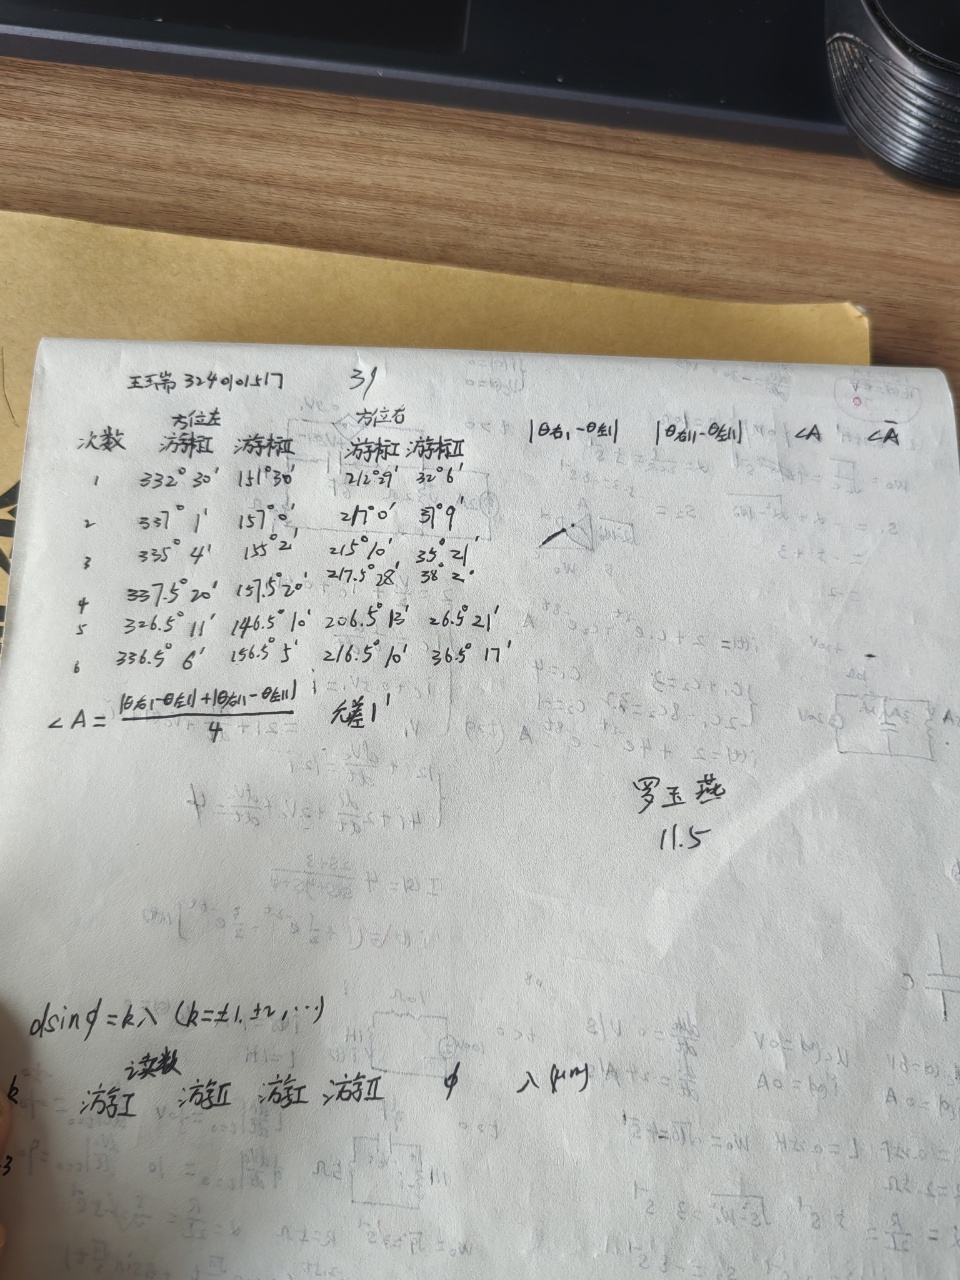
\includegraphics[width=0.8\textwidth]{figure/raw.jpg}
        \caption{原始数据记录1}
    \end{figure}
    

\section{结果与分析}

    \subsection{数据处理与结果}
    \xiaosi （列出数据表格、选择数据处理方法、给定测量或计算结果，30分）

    \small{
\begin{tabular}{|c|c|c|c|c|c|c|c|}
\hline
\multirow{2}{*}{实验次数} & \multicolumn{2}{c|}{方位左} & \multicolumn{2}{c|}{方位右} & \multirow{2}{*}{$\left|\theta_{\text{左I}} - \theta_{\text{右I}}\right|$} & \multirow{2}{*}{$\left|\theta_{\text{左II}} - \theta_{\text{右II}}\right|$} & \multirow{2}{*}{$\angle A$} \\
\cline{2-5}
& 游标I窗$\theta_{\text{左I}}$ & 游标II窗$\theta_{\text{左II}}$  & 游标I窗$\theta_{\text{右I}}$ & 游标II窗$\theta_{\text{右II}}$ &  &  &  \\
\hline
1 & $332^\circ 30'$ & $151^\circ 30'$ & $212^\circ 29'$ & $32^\circ 6'$ & $120.02^\circ$ & $119.40^\circ$ & $59.86^\circ$ \\
\hline
2 & $337^\circ 1'$ & $157^\circ 0'$ & $217^\circ 0'$ & $37^\circ 9'$ & $120.02^\circ$ & $119.85^\circ$ & $59.97^\circ$ \\
\hline
3 & $335^\circ 4'$ & $155^\circ 2'$ & $215^\circ 10'$ & $35^\circ 21'$ & $119.90^\circ$ & $119.68^\circ$ & $59.80^\circ$ \\
\hline
4 & $337.5^\circ 20'$ & $157.5^\circ 20'$ & $217.5^\circ 28'$ & $38^\circ 2'$ & $120.00^\circ$ & $119.30^\circ$ & $59.83^\circ$ \\
\hline
5 & $326.5^\circ 11'$ & $146.5^\circ 10'$ & $206.5^\circ 13'$ & $26.5^\circ 21'$ & $120.00^\circ$ & $119.82^\circ$ & $59.96^\circ$ \\
\hline
6 & $336.5^\circ 6'$ & $156.5^\circ 5'$ & $216.5^\circ 10'$ & $36.5^\circ 17'$ & $119.93^\circ$ & $119.80^\circ$ & $59.93^\circ$ \\
\hline
\end{tabular}
}

    以下写出计算公式、简要过程及计算结果。

    根据原始数据补充数据表格，$\angle A$的计算公式为
  \begin{equation}
    \angle A = \frac{\left|\theta_{\text{左I}} - \theta_{\text{右I}}\right| + \left|\theta_{\text{左II}} - \theta_{\text{右II}}\right|}{4}
\end{equation}

以第1组数据为例计算过程：
\begin{align*}
|\theta_{\text{左I}} - \theta_{\text{右I}}| &= |332^\circ30' - 212^\circ29'| = 120^\circ1' = 120.02^\circ \\
|\theta_{\text{左II}} - \theta_{\text{右II}}| &= |151^\circ30' - 32^\circ6'| = 119^\circ24' = 119.40^\circ \\
\angle A &= \frac{120.02^\circ + 119.40^\circ}{4} = 59.8552^\circ \approx 59.86^\circ
\end{align*}

$\angle A$平均值：$\bar {\angle A}= \frac{59.86+59.97+59.80+59.83+59.96+59.93}{6} = 59.89^\circ$
\subsection{误差分析}
    \xiaosi （运用测量误差、相对误差、不确定度等分析实验结果，20分）

    A类不确定度：
\begin{align*}
u_A &= \sqrt{\frac{\sum(\angle A_i - \bar{\angle A})^2}{n(n-1)}} \\
&= \sqrt{\frac{0.03^2+0.08^2+0.09^2+0.06^2+0.07^2+0.04^2}{30}} \\
&= 0.03^\circ
\end{align*}
B类不确定度：$u_B=1'=0.02 ^\circ$

合成不确定度：
$$ u_C = \sqrt{u_A^2 + u_B^2} = \sqrt{0.03^2 + 0.02^2} = 0.037^\circ $$
最终结果表达式：$$ \angle A = (59.89 \pm 0.04)^\circ $$
误差原因分析：
\begin{itemize}
\item 分光计游标读数误差（最小刻度1'）
\item 平台与望远镜未严格对准引起的系统误差。对光、调焦等分光计基本操作比较困难繁杂，第一次学习尝试难免不准确，造成了一定的误差。
\end{itemize}
    \subsection{实验探讨}
    \xiaosi （对实验内容、现象和过程的小结，不超过100字，10分）

    通过分光计测量三棱镜顶角实验，验证了自准直法的可靠性。实验中发现平台水平调节对测量精度影响显著，当十字像与叉丝严格重合时读数最准确。测量过程中需注意消除偏心差，多次测量取平均可有效减小随机误差。
\section{思考题}

    \xiaosi （解答教材或讲义或老师布置的思考题，10分）

    \subsection{如果汞灯坏了，你能想到其他方法利用分光计测量三棱镜顶角吗？}

    若汞灯损坏，可用以下方法：
\begin{itemize}
\item 改用钠灯或激光光源配合滤光片
\item 利用白炽灯+光栅产生特征谱线
\item 采用日光通过狭缝形成连续光谱
\end{itemize}
\subsection{试画出自准直法测量三棱镜顶角的光路图。}
\begin{figure}[H]
    \centering
    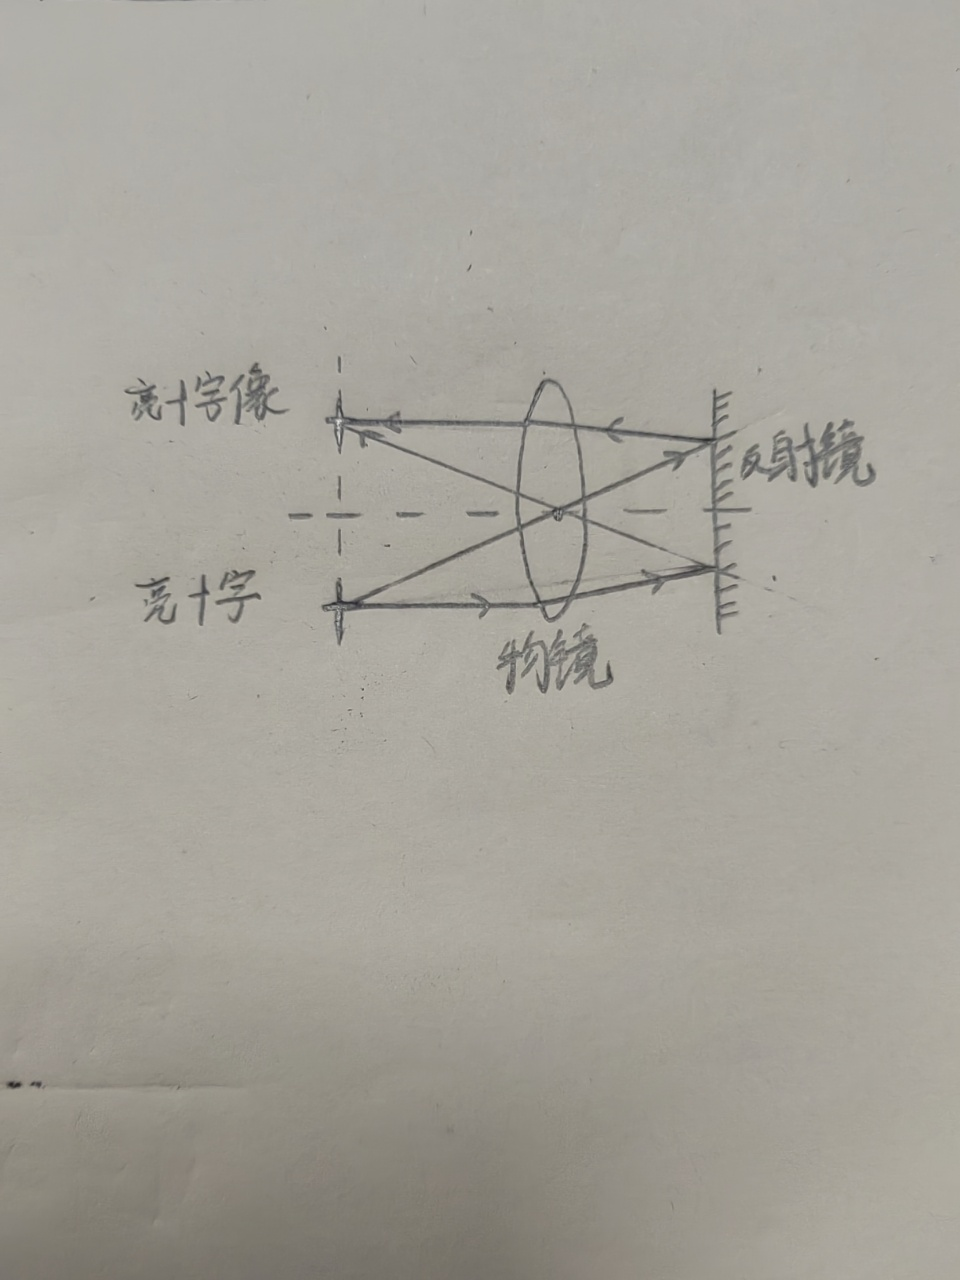
\includegraphics[width=0.6\textwidth]{figure/optical_path.jpg}
    \caption{自准直法测量三棱镜顶角的光路图}
\end{figure}
\subsection{如果望远镜中看到十字像在“十”形叉丝上刻线的上面，而当平台转过180°后看到的十字像在“十”形叉丝上刻线的下面，试问这时应该调节望远镜的倾斜度呢？还是应调节平台的倾斜度？}

应该调节平台的倾斜度。望远镜的倾斜度在平台转过180°之前已经调整完毕，不宜再移动。
\subsection{三棱镜顶角为什么应接近平台中心偏上一点点位置？}

\begin{itemize}
\item 保证反射面与望远镜光轴垂直
\item 避免棱镜自重导致平台倾斜
\item 便于同时观察两个反射面的像
\end{itemize}
\newpage

\sihao\textbf{注意事项：}
\xiaosi
\begin{enumerate}
    \item 用PDF格式上传“实验报告”，文件名：学生姓名+学号+实验名称+周次。
    \item  “实验报告”必须递交在“学在浙大”的本课程的对应实验项目的“作业”模块内。
    \item  “实验报告”成绩必须在“浙江大学物理实验教学中心网站”-“选课系统”内查询。
    \item 教学评价必须在“浙江大学物理实验教学中心网站”-“选课系统”内进行，学生必须进行教学评价，才能看到实验报告成绩，教学评价必须在本次实验结束后 3 天内进行。
\end{enumerate}

\vspace{1cm}
\xiaosi\centering \textbf{浙江大学物理实验教学中心制}

\end{document}